\documentclass{article}
\usepackage{tabularx}
\usepackage{longtable}
\usepackage{array}
\usepackage{float}
\usepackage{listings}
\usepackage{amsmath}
\usepackage{amssymb}
\usepackage{mathtools}
\usepackage{amsfonts}
\usepackage{graphicx}
\usepackage[table]{xcolor}
\setlength{\arrayrulewidth}{0.5mm}
\graphicspath{ {./images/} }
\usepackage[margin=20mm]{geometry}
\renewcommand{\labelenumii}{\theenumii}
\renewcommand{\theenumii}{\theenumi.\arabic{enumii}.}
\renewcommand{\arraystretch}{1.5}
\newcommand{\f}[2]{f_{#1}(#2)}
\newcommand{\code}[1]{\texttt{#1}}
\DeclarePairedDelimiter{\ceil}{\lceil}{\rceil}
\DeclarePairedDelimiter{\set}{\left\{}{\right\}}
\DeclarePairedDelimiter{\parens}{\lparen}{\rparen}
\title{HW3 Report}
\date{}
\begin{document}
\maketitle
\section*{Section 1}
\subsection*{Q1:}
    \begin{figure}[H]
        \centering
        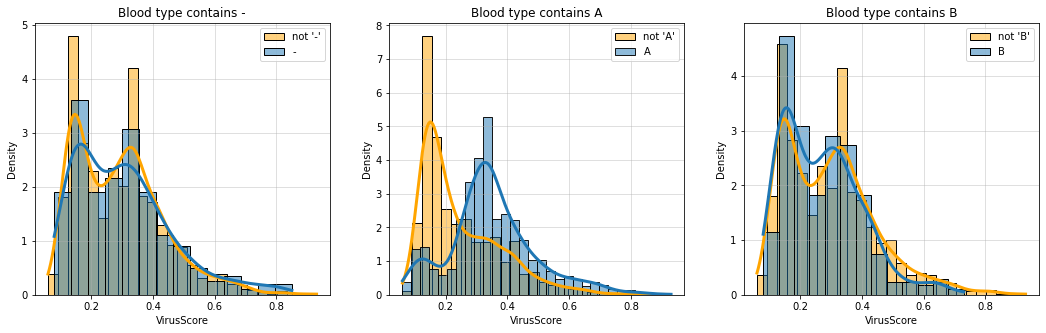
\includegraphics[scale=0.5]{images/q1.png}
        \caption{KDE plots of \code{VirusScore} conditioned different conditions of \code{blood\_type}}
        \label{fig:q1}
    \end{figure}
\subsection*{Q2:}
    \paragraph*{}
    In figure \ref{fig:q1} in the plot of A versus not A, we observe that the groups of patients with and and without "A" in their blood types are mostly seperable along a boundary that is approximately the \code{VirusScore} of $0.225$. 
    \paragraph*{}
    Therefore, the condition of contains/does not contain A would be most informative for learning \code{VirusScore}.
    As it turns out, we decided already in hw1 to create this feature.
\subsection*{Q3:}
    \begin{figure}[H]
        \centering
        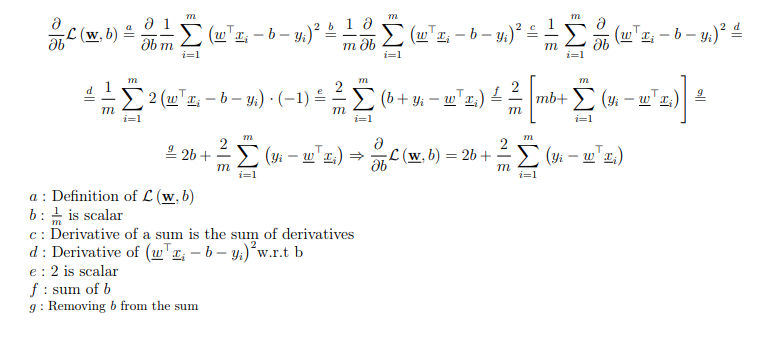
\includegraphics[scale=0.7]{images/q3.png}
    \end{figure}
\subsection*{Q4:}
    \begin{figure}[H]
        \centering
        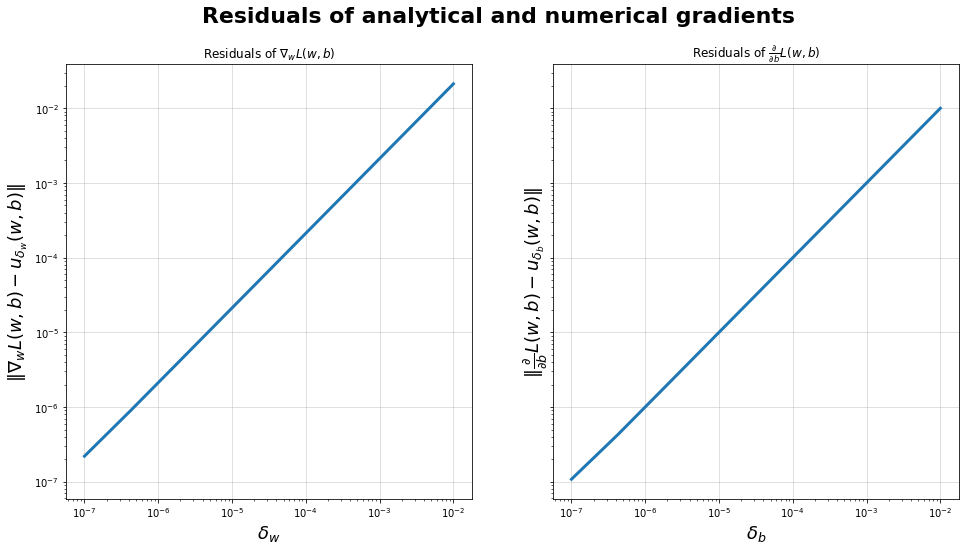
\includegraphics[scale=0.48]{q4.png}
        \caption{Plot of Residuals of analytical and numerical gradients}
        \label{fig:q4}
    \end{figure}
    \paragraph*{}
    As we can see in figure \ref{fig:q4}, the difference between the analytic and numerical gradients increases in a  monotonic fashion as the value of $\delta$ increases. This is logical, as $\delta$ is the differential size used in the definition of the numerical gradient, and therefore a smaller $\delta$  equates to a more precise estimation of the analytic gradient by the numerical gradient.
\subsection*{Q5:}
    \begin{figure}[H]
        \centering
        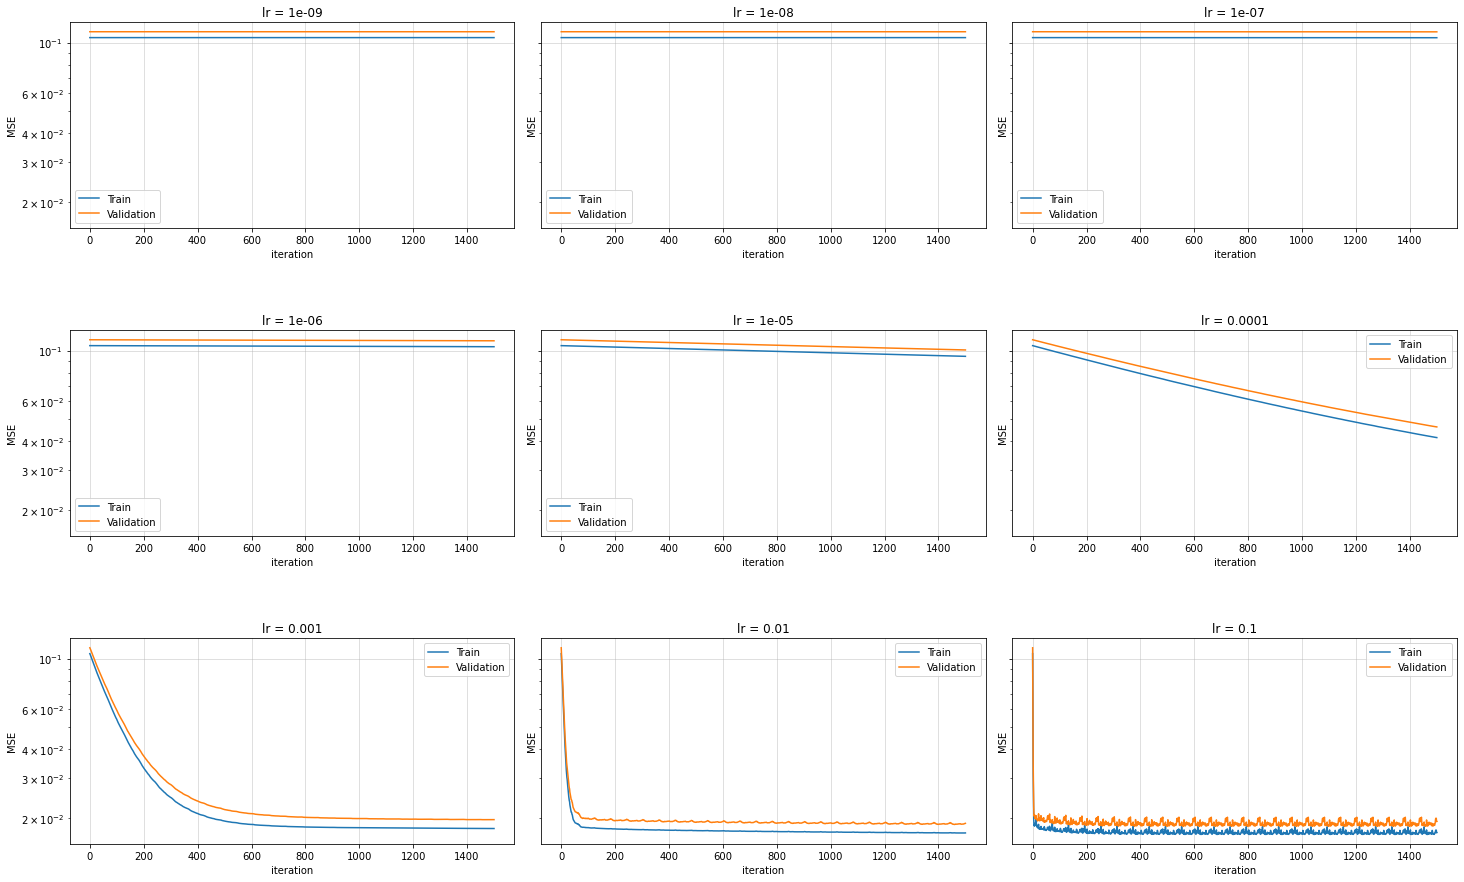
\includegraphics[scale=0.35]{q5.png}
        \caption{Graphs of Training and Validation Losses as Functions of Iteration Number for Different  Learning Rates}
        \label{fig:q5}
    \end{figure}
    \paragraph*{}
    We can see in figure \ref{fig:q5} that for smaller lr, for those that converge, the convergence is at a higher loss for both the training and validation. This matches the theory, since if the lr is too small, the SGD algorithm is likely to converge to a sub-optimal solution. In addition we observe that for the lr equal to $0.1$ the graphs do not converge for both training and validation losses and for lr equal to $0.01$ the validation loss does not converge, which fits the theory that says that learning rates that are too high are likely to cause the SGD algorithm to take steps that are too large and thus repeatedly skip-over the optimal solution. This points to $0.001$ as being the optimal lr, as both the validation and training losses converge to values that are substantially lower than the next smaller lr.
\subsection*{Q6:}
    \begin{center}
        \begin{tabular}{|c|c|c|c|}
            \hline
            \rowcolor{gray!60}
            Model & Section & Train MSE & Valid MSE\\ \hline
            \rowcolor{gray!20}
            ~&~ & \multicolumn{2}{c|}{Cross Validated}\\ \hline
            Dummy & 3 & $0.0204$ & $0.0205$\\ \hline
        \end{tabular}
    \end{center}
\section*{Section 4}
\subsection*{Q8:}
    \begin{center}
        \begin{tabular}{|c|c|c|c|}
            \hline
            \rowcolor{gray!60}
            Model & Section & Train MSE & Valid MSE\\ \hline
            \rowcolor{gray!20}
            ~&~ & \multicolumn{2}{c|}{Cross Validated}\\ \hline
            Dummy & 3 & $0.0204$ & $0.0205$\\ \hline
            Ridge linear & 4 & $0.0204$ & $0.0205$\\ \hline
        \end{tabular}
    \end{center}
\section*{Section 6}
\subsection*{Q16:}
    \paragraph*{}
    When using a polynomial feature mapping, we can expect the training error to decrease and the validation error to increase. This is because the polynomial mapping will give more flexibility to the regression model to more closely try to fit the training data during training in a polynomial way, thereby leading to lower training error, but also causing overfitting and therefore leading to a higher validation error.

\end{document}